% This is a model template for the solutions in computational science. You can find a very useful documentation for LaTeX in Finnish at ftp://ftp.funet.fi/pub/TeX/CTAN/info/lshort/finnish/ or in English at ftp://ftp.funet.fi/pub/TeX/CTAN/info/lshort/english/. The section List of mathematical symbols in Chapter 3 is especially useful for the typesetting of mathematical formulas.

% Compile the document to PDF by command 'pdflatex model.tex' in the terminal. The command must be run twice for the references in the text to be correct.

\documentclass[a4paper,11pt]{article}
\usepackage[utf8]{inputenc}
% This includes letters such as � and �
\usepackage[T1]{fontenc}
% Use here 'Finnish' for Finnish hyphenation. You may have to compile the code twice after the change. 
\usepackage[english]{babel}
\usepackage{graphicx}
% Some math stuff
\usepackage{amsmath,amsfonts,amssymb,amsbsy,commath,booktabs,hyperref}  
% This is just to include the urls
\usepackage{hyperref,subcaption}
\usepackage[margin=2cm]{geometry}

\setlength{\parindent}{0mm}
\setlength{\parskip}{1.0\baselineskip}
\usepackage{minted}
\usemintedstyle{tango}

\usepackage{listings}
\usepackage{color}
\usepackage{pdfpages}
\DeclareMathAlphabet{\pazocal}{OMS}{zplm}{m}{n}

\definecolor{dkgreen}{rgb}{0,0.6,0}
\definecolor{gray}{rgb}{0.5,0.5,0.5}
\definecolor{mauve}{rgb}{0.58,0,0.82}

\lstset{frame=tb,
	language=Python,
	aboveskip=3mm,
	belowskip=3mm,
	showstringspaces=false,
	columns=flexible,
	basicstyle={\tiny\ttfamily},
	numbers=none,
	numberstyle=\tiny\color{gray},
	keywordstyle=\color{blue},
	commentstyle=\color{dkgreen},
	stringstyle=\color{mauve},
	breaklines=true,
	breakatwhitespace=true,
	tabsize=4
}

\begin{document}

\title{CS-E4830 Kernel Methods in Machine Learning \\ Assignment 1} % Replace the exercise round number
\author{Kunal Ghosh, 546247} % Replace with your name and student number
\maketitle
\section{Solution to Question 1}
\subsection{(a) True}
Its given that $K_1$ and $K_2$ are Positive semi-definite matrices. So, for any vector $v$ we have
\begin{equation}
    \begin{split}
        & v^{T}K_1v \ge 0 \text{ and } v^{T}K_2v \ge 0\\
        \text{from question } K & = aK_1 + bK_2 \text{ where } a,b \in \pazocal{R}^+ \\ 
        \text{then, } v^TKv &= v^T (aK_1 + bK_2) v \\
        & = v^T (aK_1) v + v^T (bK_2) v \\
        & = a (v^TK_1v) + b (v^TK_2)v \\
        & \text{Since, } a,b > 0 \text{ and } v^TK_1v, v^TK_2v \ge 0\\
        & \implies a (v^TK_1v) + b (v^TK_2)v \ge 0 \\
        & \implies  v^T (aK_1 + bK_2) v \ge 0 \\
        & \implies v^TKv \ge 0 \\
    \end{split}
\end{equation}
So, $K$ is Positive semi-definite. Hence a Kernel Matrix.
\subsection{(b) False}
If matrix $K$ is defined as ${K = K_1 - K_2}$, where ${K_1 , K_2}$ are positive semi-definite matrices, then
\begin{equation}
    \begin{split}
        v^TKv &= v^T(K_1 - K_2)v \\
        &= v^T(K_1)v - v^T(K_2)v \\
    \end{split}
\end{equation}
We know that, ${ v^TK_1v, v^TK_2v \ge 0 }$. However, the difference of two non-negative numbers is not always non-negative.
\begin{equation}
    \begin{split}
        & \implies v^T(K_1)v - v^T(K_2)v \ngeq 0 \\
        & \implies v^TKv \ngeq 0 \\
    \end{split}
\end{equation}

Hence ${K = K_1 - K_2}$ is not always positive semi-definite. Hence $K$ need not be a Kernel Matrix.
\subsection{(c) False}
If matrix $K$ is defined as ${K = K_1K_2}$ where ${K_1 , K_2}$ are positive semi-definite matrices, then\\
\textbf{[Counter Example]} : Product of two symmetric matrices is not always symmetric. \\
for, ${K_1 =
\begin{bmatrix}
       1 & -1 \\[0.3em]
       -1 & 1 \\[0.3em]
\end{bmatrix}
}$ and ${K_2 =
\begin{bmatrix}
       -2 & 1 \\[0.3em]
       1 & -3 \\[0.3em]
\end{bmatrix}
}$

where $\text{det}(K_1) > 0$ and $\text{det}(K_2) > 0$ so all the eigen values of $K_1$ and $K_2$ are positive. 
Hence $K_1$ and $K_2$ are positive semi-definite matrices. But, \\${K = K_1K_2 = 
\begin{bmatrix}
       -3 & 4 \\[0.3em]
       3 & -4 \\[0.3em]
\end{bmatrix}
}$\\
is not a symmetric matrix. Therefore ${K = K_1K_2}$ need not be a Kernel Matrix.
\subsection{(d) False}
\textbf{[Counter Example]} : Examples of $K_1$ and $K_2$ given above (previous section) are valid Kernel Matrices but don't have all positive entries.
\subsection{(e) True}
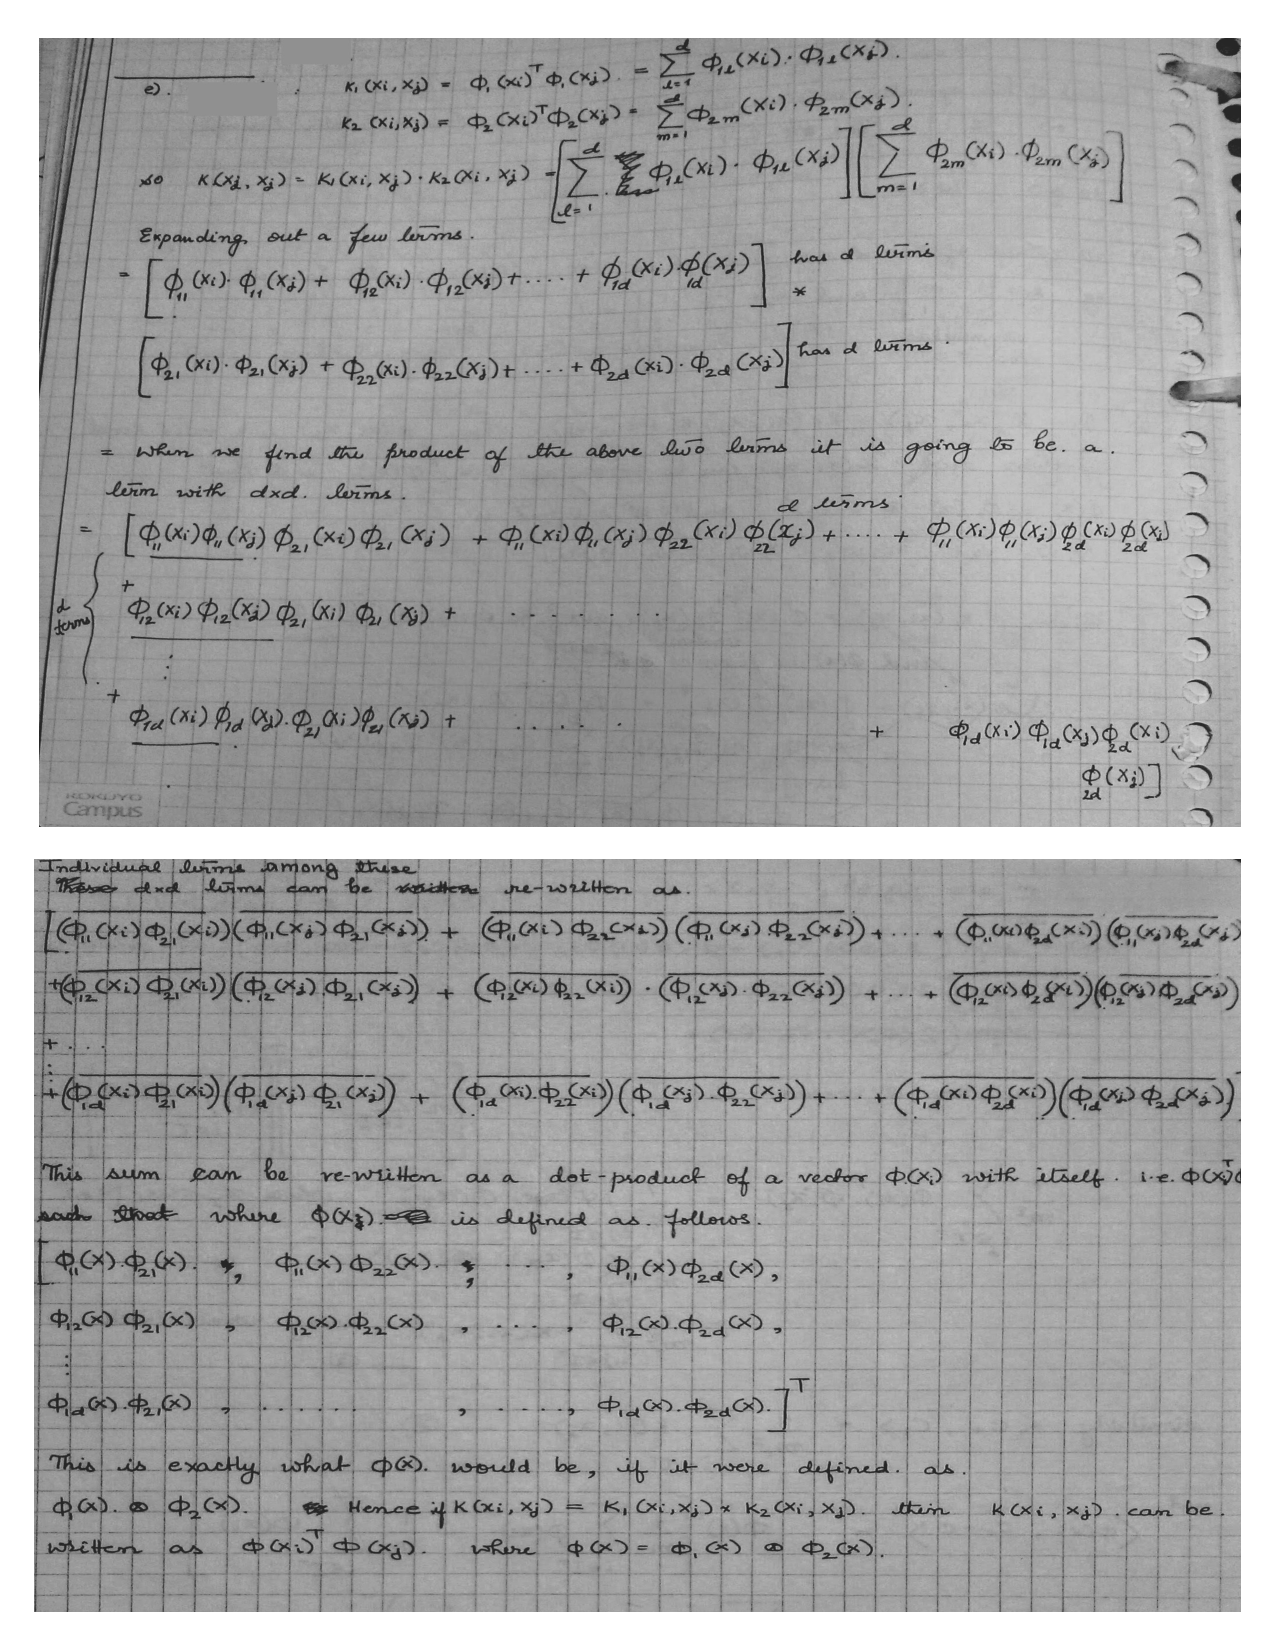
\includepdf[pages=-,scale=1]{1_5.pdf}
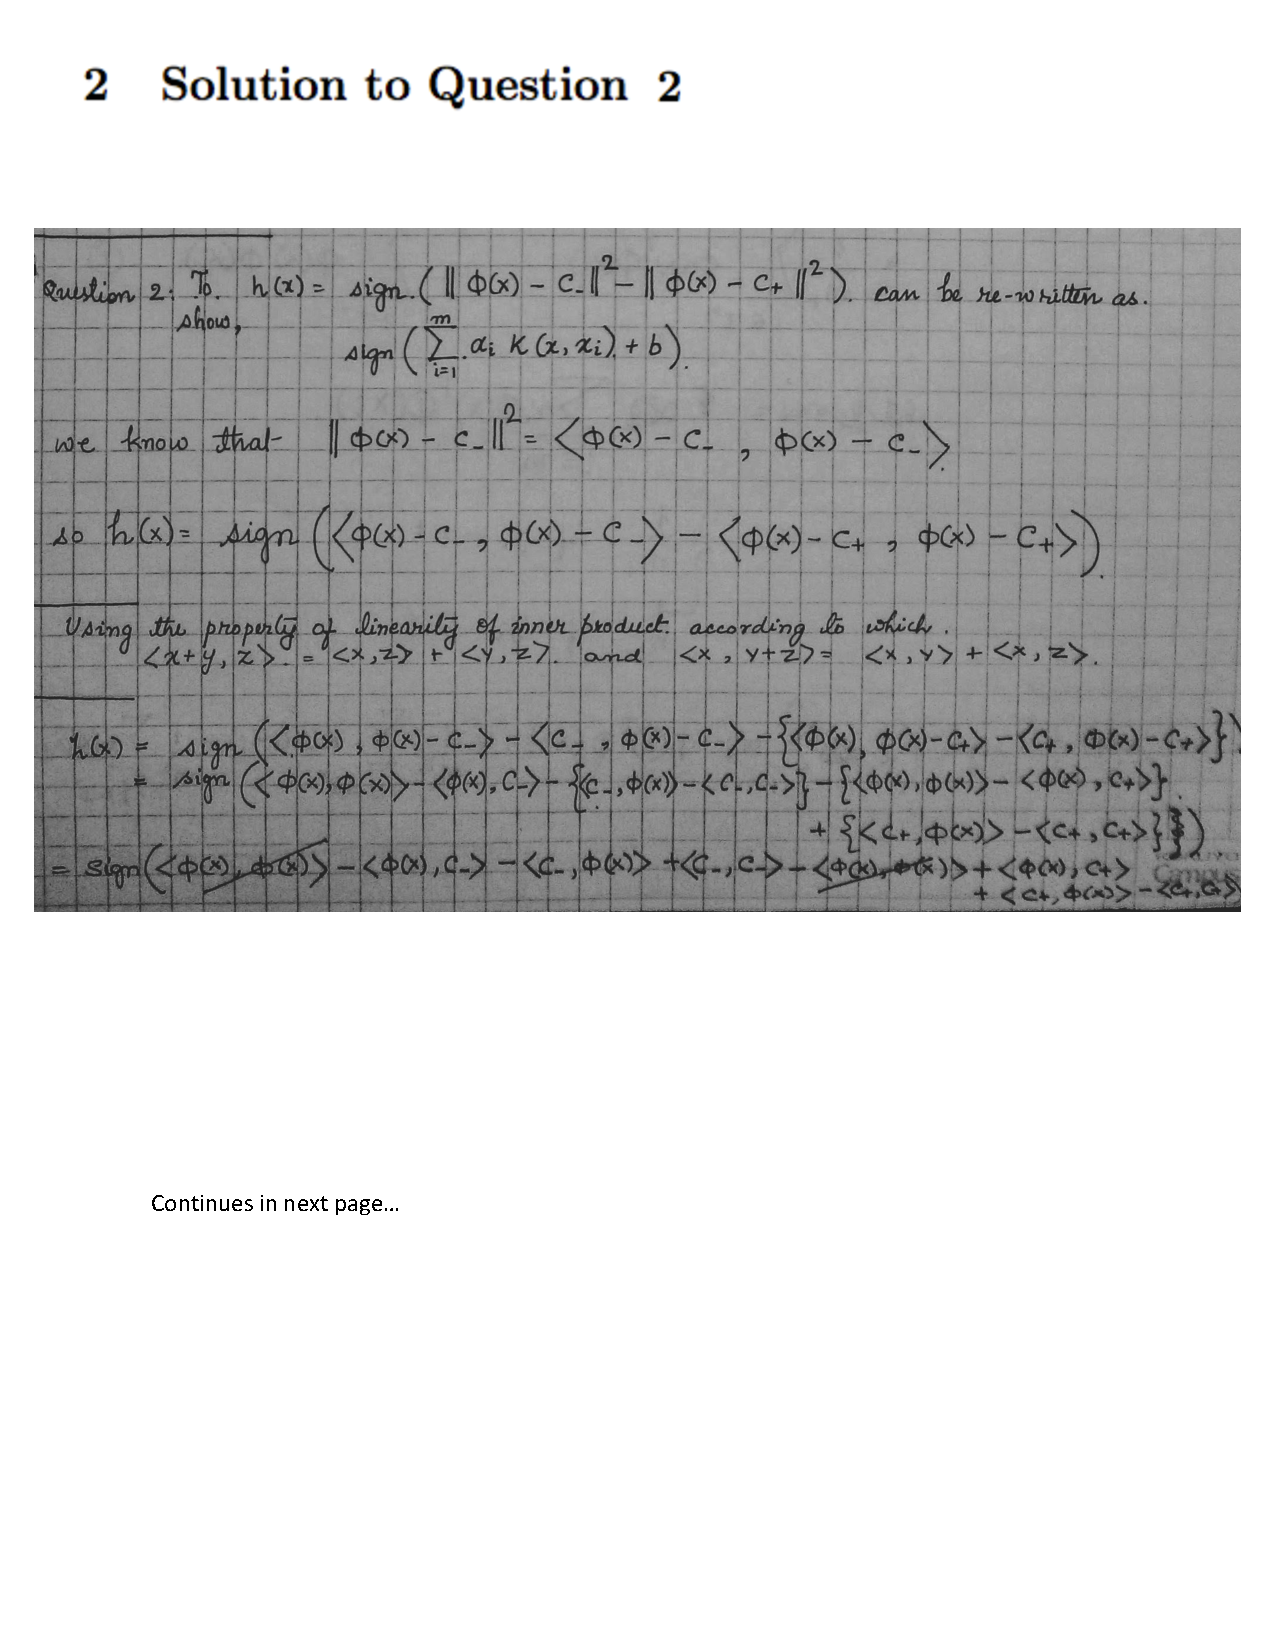
\includepdf[pages={1,2},scale=1]{2.pdf}
\section{Solution to Question 3}
\inputminted[baselinestretch=1, fontsize=\small, breaklines=true]{octave}{../gaussian_kernel.m}
\section{Solution to Question 4}
\inputminted[baselinestretch=1, fontsize=\small, breaklines=true]{octave}{../parzen_classify.m}
\section{Solution to Question 5}
In the caption in the figures below $\sigma$ is a parameter of the gaussian kernel which is used for the task of classification in this problem. Among the figures, fig-\ref{fig:1} shows the learning curves and fig-\ref{fig:2} shows the decision boundary for various values of $\sigma$. More description in the captions of the figures.
\begin{figure}[ht!]
    \centering
    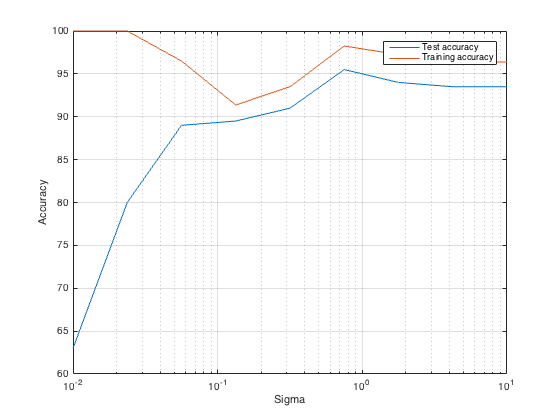
\includegraphics[scale=0.7]{learning_curves.png}
    \caption{Learning curves: Initially, with low values of sigma there is overfitting (high training accuracy, low test accuracy) as the sigma values increase the model generalizes better until sigma reaches $\approx 0.7$ then the model starts to underfit.}
    \label{fig:1}
\end{figure}
\begin{figure}[ht!]
    \centering
    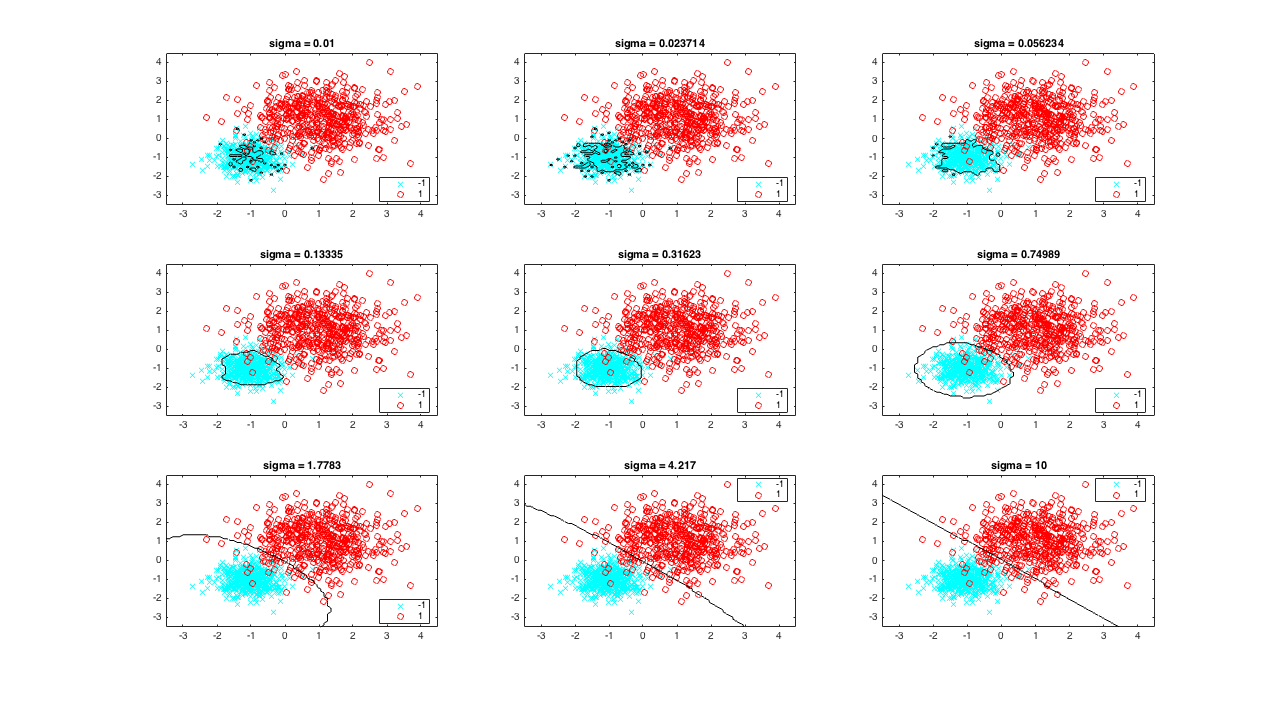
\includegraphics[scale=0.4]{sigma_figs.png}
    \caption{Decision Boundaries: For low values of sigma overfitting is clearly visible (small "circles" tightly encircling certain datapoints). As the sigma increases the model generalizes better, for $\sigma \approx 0.7$ the test accuracy is the best (least number of red-circles inside the decision boundary). Finally, as the sigma keeps on increasing the decision boundary tends to a linear decision boundary which isn't the most ideal for this dataset as can be seen in the learning curves Fig-\ref{fig:1} above where both the training and test accuracy drops as the sigma is increased beyond $\approx$ 0.7.}
    \label{fig:2}
\end{figure}
\end{document}

   

